% This .tex file (and associated .cls) produces:
%       1) The Permission Statement
%       2) The Conference (location) Info information
%       3) The Copyright Line TSConIT
%       4) NO page numbers
%       5) NO headers and/or footers
%
% Using 'sig-alternate.cls' you have control, however, from within
% the source .tex file, over both the CopyrightYear
% (defaulted to 200X) and the ACM Copyright Data
% (defaulted to X-XXXXX-XX-X/XX/XX).
% e.g.
% \CopyrightYear{2007} will cause 2007 to appear in the copyright line.
% \crdata{0-12345-67-8/90/12} will cause 0-12345-67-8/90/12 to appear in the copyright line.
%
% ---------------------------------------------------------------------------------------------------------------
% This .tex source is an example which *does* use
% the .bib file (from which the .bbl file % is produced).
% REMEMBER HOWEVER: After having produced the .bbl file,
% and prior to final submission, you *NEED* to 'insert'
% your .bbl file into your source .tex file so as to provide
% ONE 'self-contained' source file.
%

% refers to the cls file being used
\documentclass{sig-alternate-br}
\usepackage{float}
\usepackage{caption}
\usepackage{subcaption}
\usepackage{hyperref}
\usepackage{tabularx}
\usepackage{graphicx}
\restylefloat{figure}
\restylefloat{table}
\begin{document}

%
% --- Author Metadata here --- DO NOT REMOVE OR CHANGE 
%\conferenceinfo{13$^{th}$ Twente Student Conference on IT}{June 23$^{st}$, 2010, Enschede, The Netherlands.}
\CopyrightYear{2015} % Allows default copyright year (200X) to be over-ridden - IF NEED BE.
%\crdata{0-12345-67-8/90/01}  % Allows default copyright data (0-89791-88-6/97/05) to be over-ridden - IF NEED BE.
% --- End of Author Metadata ---

\title{Micro Data Server using Raspberry Pi for Video Streaming}
% In Bachelor Referaat at University of Twente the use of a subtitle is discouraged.
 \subtitle{Research Proposal}

\numberofauthors{1} 
\author{ 
% You can go ahead and credit any number of authors here,
% e.g. one 'row of three' or two rows (consisting of one row of three
% and a second row of one, two or three).
%
% The command \alignauthor (no curly braces needed) should
% precede each author name, affiliation/snail-mail address and
% e-mail address. Additionally, tag each line of
% affiliation/address with \affaddr, and tag the
% e-mail address with \email.
%
% 1st. author
\alignauthor P.J.E. Velthuis\\
       \affaddr{University of Twente}\\
       \affaddr{P.O. Box 217, 7500AE Enschede}\\
       \affaddr{The Netherlands}\\
       \email{p.j.e.velthuis@student.utwente.nl}
% 2nd. author
\alignauthor 2nd Author\\
       \affaddr{2nd author's affiliation}\\
       \affaddr{1st line of address}\\
       \affaddr{2nd line of address}\\
       \email{2nd author's email address}
% 3rd. author
\alignauthor 3rd Author\\
       \affaddr{3rd author's affiliation}\\
       \affaddr{1st line of address}\\
       \affaddr{2nd line of address}\\
       \email{3rd author's email address}
}

%\additionalauthors{Additional authors: John Smith (The
%Th{\o}rv{\"a}ld Group, email: {\texttt{jsmith@affiliation.org}})
%and Julius P.~Kumquat (The Kumquat Consortium, email:
%{\texttt{jpkumquat@consortium.net}}).}
%\date{30 July 1999}

\maketitle
\begin{abstract}
This document describes a research proposal in the
area of cloud computing services. Cloud computing is a trend IT that customers move computing and data away from desktop and portable PCs into large data centers. These data centers require a lot of power and cooling. Nowadays 30 \% of the data coming from these data centers is video streaming. The Raspberry Pi is a device that might improve these problems. The main research question
is therefore: Is it possible to improve availability algorithms for video streaming by using small scale Raspberry Pi’s data center? To answer this question a micro Raspberry Pi video streaming service will be build. 
\end{abstract}

\keywords{Cloud computing, Raspberry Pi, micro data server, video streaming, load balancing}

\section{Motivation}
The amount of cloud computing services is increasing fast \cite{armbrust:2009}. But despite the attention from the research community, research and development of Cloud Computing services is still in its early days~\cite{tso:2013}. \newline
Cloud computing is a trend IT that customers move computing and data away from desktop and portable PCs into large data centers \cite{dikaiakos:2009}. In the future most internet users access internet services over lightweight portable devices. This requires a lot of data bandwidth. Video streaming is something that requires a lot of bandwidth. This bandwidth usage causes bottlenecks and small data servers can be build after these bottlenecks. This makes research on this topic very interesting.  \newline
In this research a small data server consisting of Raspberry Pi´s will be investigated. A reason for this is that data centers require a lot of space and cooling. There are now new technologies such as for example the powerful ARM processor. Many companies want to explore the possibilities of for example the Raspberry Pi and his ARM Processor \cite{Pcextreme}. Some data centers already offer some cloud computing using the Raspberry Pi. A reason for this is the small location that the Raspberry Pi needs, and the low power usage of a Raspberry Pi \cite{hosting,Pcextreme}. A Raspberry Pi has a power usage between the 3-5 Watt. A normal server has a power usage between the 75 and 250 Watt~\cite{Powerusage,beloglazov2012energy}. However the Raspberry Pi has less computing power then a normal server. The low power consumption and its computing power could mean that it is better to use a Raspberry Pi for specific small tasks that do not demand a whole server. During this research there will be a investigation on the performance of the Raspberry Pi as a small data server. \newline
A Raspberry Pi can be the small data center for the future \cite{tso:2013}. The Raspberry is a relatively cheap device for 40 euro. This makes it cheaper to do research in compared to a normal server.  Building a cloud like this can be a cost effective scale model\cite{tso:2013}. It's a ideal testbed for testing distributed software. 


\section{Specific problem}

The Netherlands have one million subscribers for Netflix \cite{volkskrant}. Netflix is a popular video streaming service that makes HD movies watching possible. For this Netflix makes use of a content distribution network (CDN). On the internet this is known as a on demand service \cite{Adhikari:2012}. Netflix makes use of MPEG-DASH a protocol that makes streaming over HTTP possible \cite{martin:2013}. The problem is that Netflix is responsible for  29.7\% of the peak downstream traffic in US \cite{Adhikari:2012}. \newline
In the Netherlands more and more users are making use of video streaming as Youtube and Netflix. This makes it interesting to do more research in video streaming by cloud computers. Most of the research nowadays happen on expensive large servers \cite{tso:2013}. For this it can be very useful to see if it is possible to do research on a small computer like a Raspberry Pi. The problem is that we do not know if video streaming on a small raspberry pi cluster is possible. 

\section{Research questions}
The main research question
\begin{center} 
Is it possible to improve availability algorithms for video streaming by using small scale Raspberry Pi’s data center? \end{center}
This research will be part literature study and a part of it will be building a small Raspberry Pi cloud to measure the availability of the video streaming. Here below there are several questions to come to a good answer for the main research question. 
\newline \newline
\subsection{Why are small scale data centers being used?}
In this research there will be a small scale cloud data center with the Raspberry Pi. The main motivation behind this is that it is ways to expensive to simulate large scale cloud computing. Resources for this motivation:
\cite{southampton, Powerusage, cox:2014} \newline
Another reason is the small location that is needed using a small scall data center. On the size of the data center is currently done a lot of research \cite{Pcextreme}. \newline
Small scale cloud computing is cloud computing with smaller computation amounts than normal. This can mean that it is better for different tasks. More motivation is that it does not use a lot cooling and power \cite{tso:2013}. Resources available for small scale cloud computing:
\cite{Pcextreme,armbrust:2009,richardson:2012,abrahamsson:2013,southampton, tso:2013, beloglazov:2010, qian:2009, hofer:2011, drago2012inside, dropbox, owncloud, Miettinen:2010:EEM:1863103.1863107, beloglazov2012energy,cox:2014} 
 
\subsection{Is it useful to use Raspberry Pi’s for video streaming?}
 The Netherlands have one million subscribers for Netflix \cite{volkskrant}. Netflix is a video streaming service that makes HD movies watching possible. This requires a lot of internet bandwidth and it could be useful to do the streaming in small scale data centers nearby. To investigate what Netflix really is there are the following resources:
\cite{volkskrant, Adhikari:2012} \newline
Netflix makes use of MPEG-DASH a protocol that makes streaming over HTTP possible. In this research there will be an investigation in the video streaming as a cloud service in a small scale data center. To investigate what that is there are the following resources:
\cite{raspberry-video,video-1080p, plissonneau:2012, computer-networking}

\subsection{What is the perfect setup for a Raspberry Pi video streaming cluster?}
This research question will look into previous cloud cluster projects: 
\cite{abrahamsson:2013,southampton, tso:2013, beloglazov:2010,cox:2014} \newline
From this a perfect setup for the hardware of the Raspberry Pi's will be build. There will be taken a look into the different software that has to be used. For example: 
\cite{raspberry-video,video-1080p, permission, nmon,bandwidth,ab} 

\subsection{How does the availability change using different load balancing techniques with the Raspberry Pi?}
With this subquestion we will look into the different load balancing techniques. In a video streaming service it's very important to have high performance and availability. That's why it's interesting to do more research on this. Resources for load balancing on Raspberry Pi:
\cite{nginx-load-balancing,nginx-load-balancing-2, nginx-load-balancing-3, Raspberry-media-server, dropbox-clone} \newline
Things that are interesting to look into are for example bandwidth usage, power usage, i/o throughput. For this the following resources will be used: 
\cite{nmon,bandwidth,ab}

\section{Research Methods}
This research will investigate a cloud computer consisting of Raspberry Pi's. The research method for this would be the Design Science research method. this is a method to solve field problems. This research will make use of the design Science method proposed by Hevner~\cite{hevner:2007}. 
\begin{figure}[H]
	\centering 
	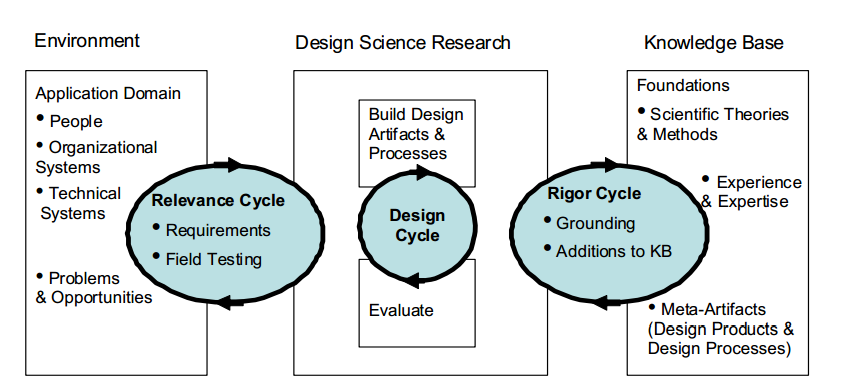
\includegraphics[width=0.4\textwidth]{Design_science.png}
	\caption{Design Science}
	\label{fig:design} %always place your label after your caption!
\end{figure}
For this design research the research will specify the requirements, existing solutions, new solutions and the result of this new solution. After that a conclusion will be given. 

\section{Research approach}
\begin{figure}[H]
	\centering 
	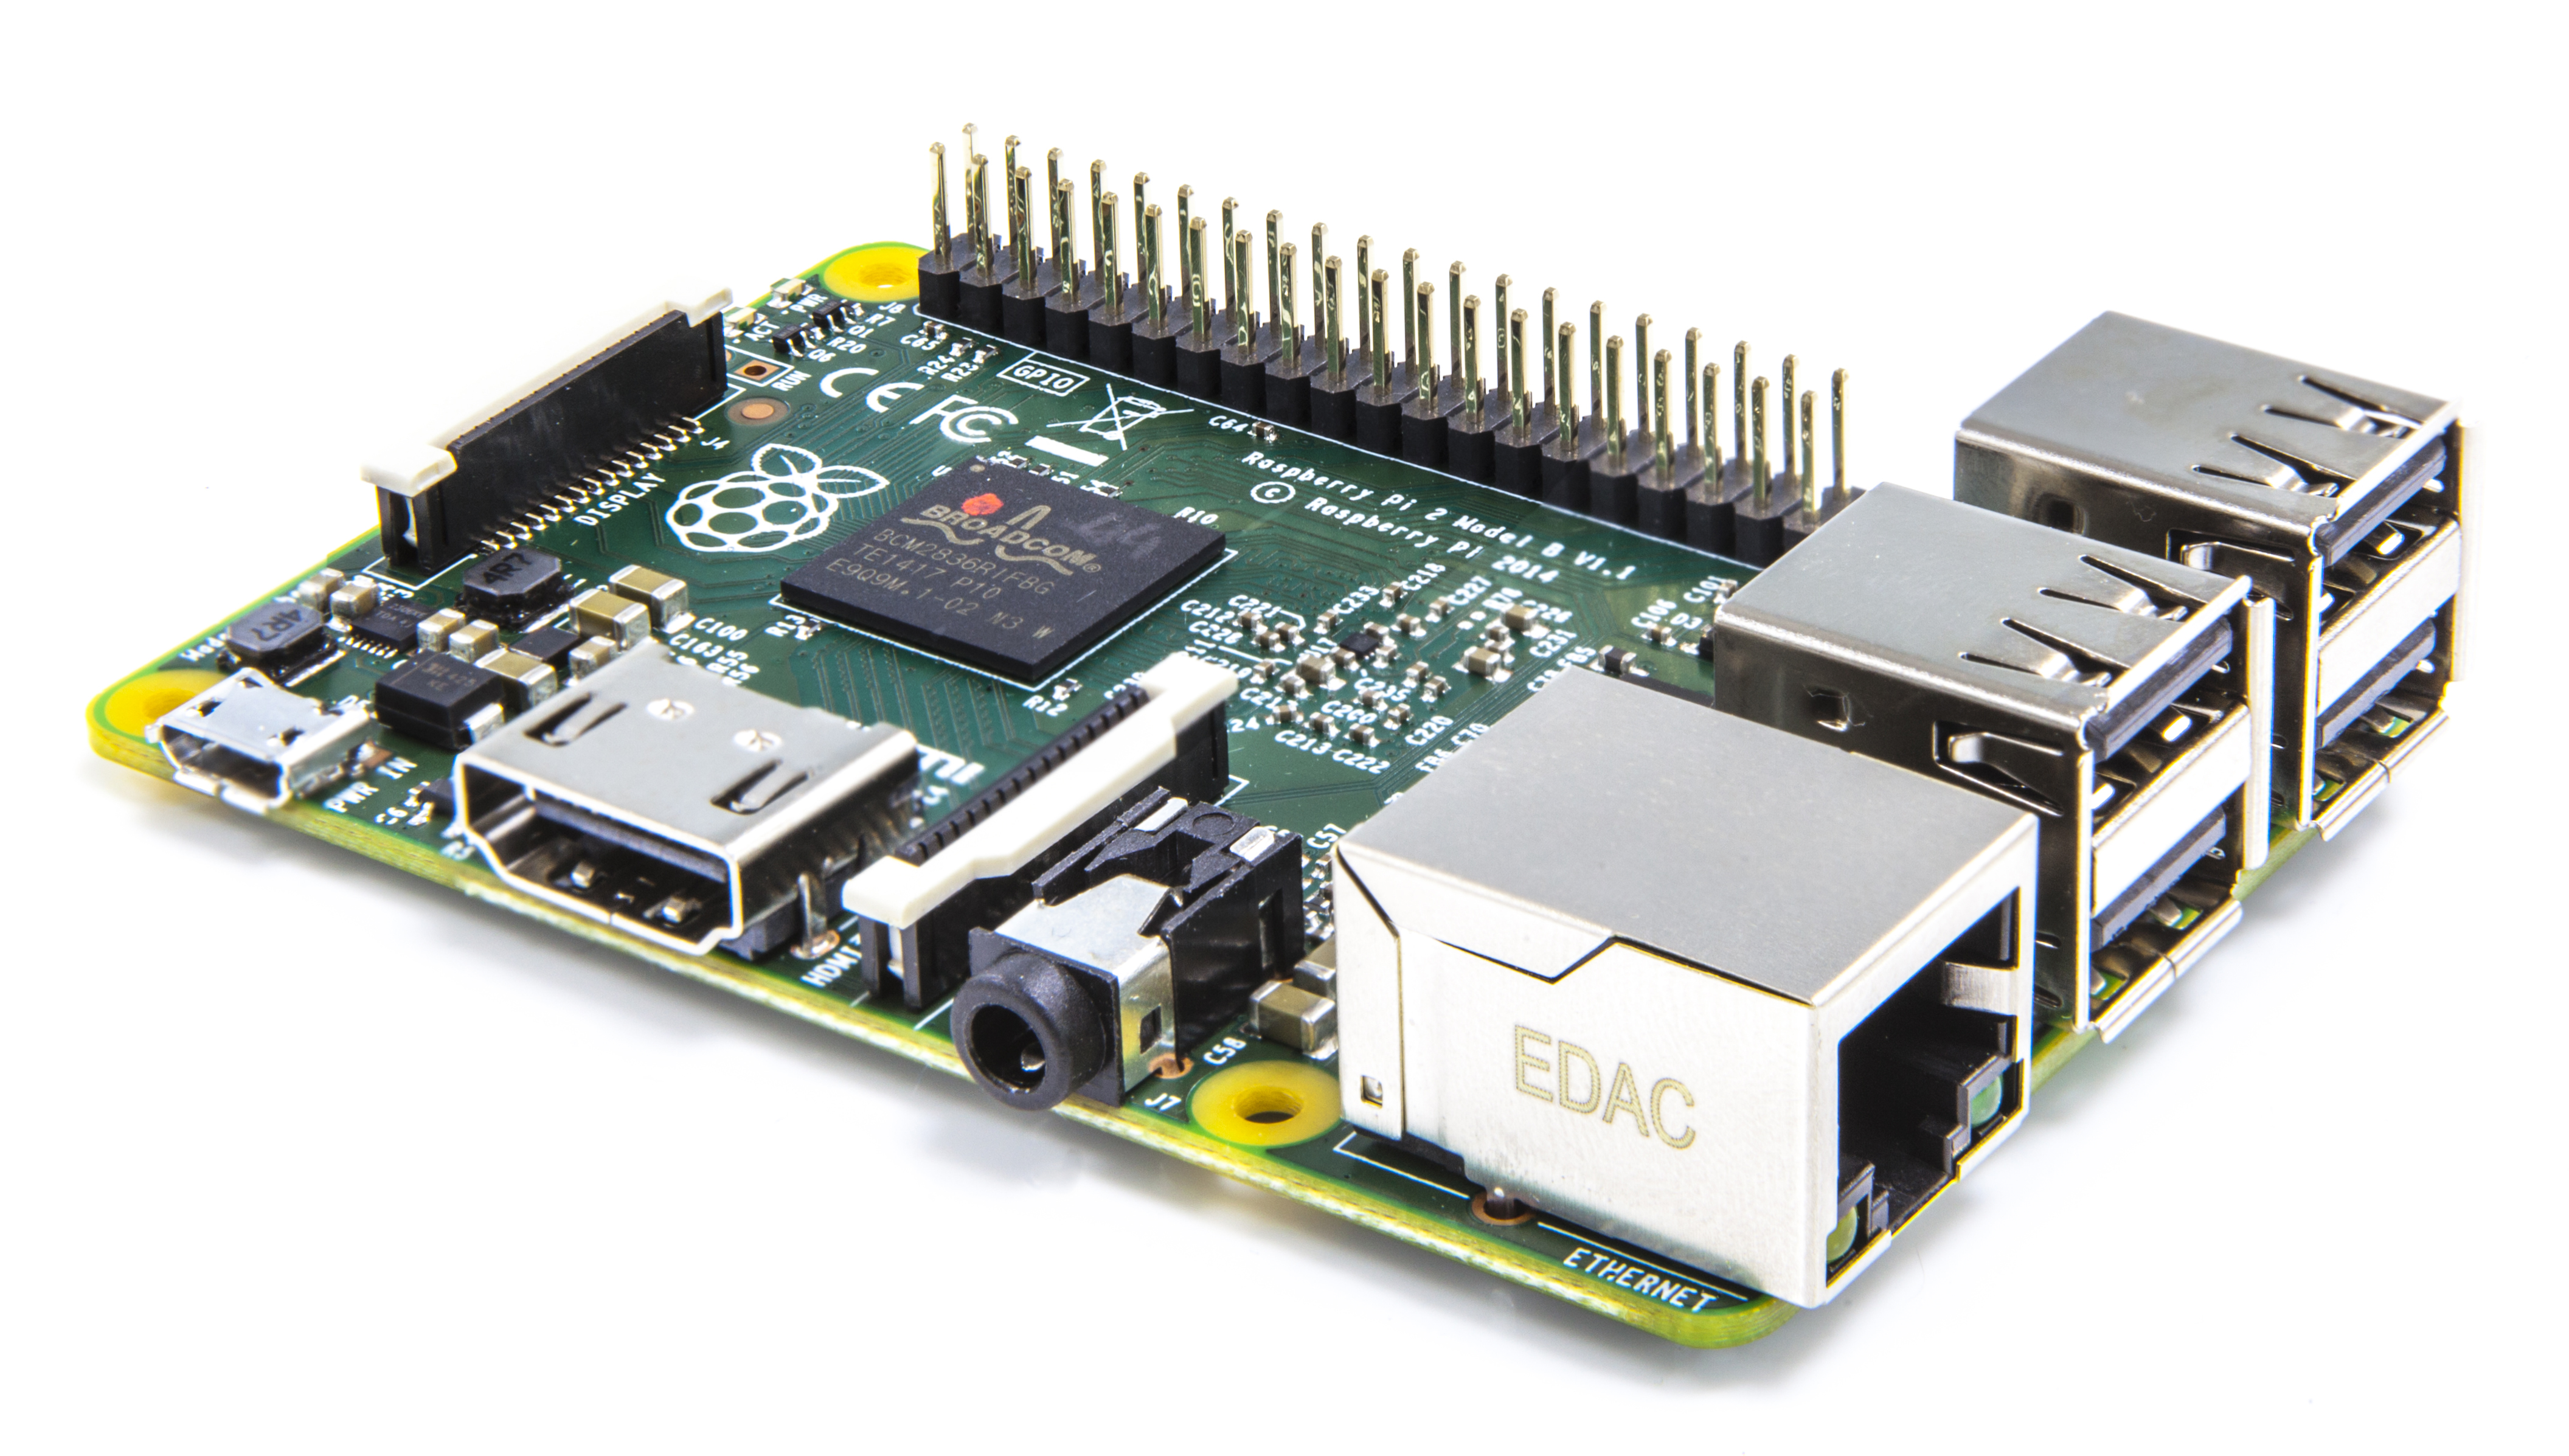
\includegraphics[width=0.4\textwidth]{Pi2ModB1GB_-comp.jpeg}
	\caption{Raspberry Pi 2 model B}
	\label{fig:raspberry} %always place your label after your caption!
\end{figure}
\begin{table}[H]
	\centering \caption{Specificaties}
	\begin{tabular}{|c|c|} \hline
		Ethernet & 100 MBps \\ \hline
		USB & 4 x USB 2.0 \\ \hline
		Video out & HDMI 1.4 \\ \hline
		Audio & 2 x analog \\ \hline
		CPU & 900MHz quad-core ARM Cortex-A7 \\ \hline
		card slot & Micro SD  \\ \hline
	\end{tabular}
	\label{tab:Specificaties}
\end{table}
For the experiment we need a Raspberry Pi B or Raspberry Pi 2 that can make use of the Ethernet. This is because a Raspberry Pi can be used as a webserver and this is needed to have this in order to make video streaming possible. This webserver will make video streaming possible. Beside the Raspberry Pi a several other things will be needed. For this we have a cost structure:
\begin{table}[H]
	\centering 
	\caption{Cost summary \cite{iapc}}
	\begin{tabular}{|c|c|c|c|c|c} \hline
		Device & cost piece& use & amount & total cost \\ \hline
		Raspberry 
		Pi 2 & 39,50 & cloud cluster & 8 & 316  \\ \hline
		UTP kabel & 1,10 & data kabel & 8 & 8,80  \\ \hline
		Micro usb kabel&1 & charging & 8 & 8  \\ \hline
		switch & 40 & internet & 1 & 40  \\ \hline
		& & & &  372,80  \\ \hline
	\end{tabular}
	\label{tab:cost}
\end{table}

So first he video streaming webserver will be made. 
After this we will make a cluster with one Raspberry Pi as a load balancer and the other two as a video stream pi. The university of Southampton has made a cluster possible \cite{southampton}. So I think it is also possible for video streaming. With this there several performance tests can be done. For example some test in streaming in different quality with load balancing. The setup of the raspberry Pi can be seen in the figure below ~\ref{fig:setup}.

\begin{figure}[H]
\centering 
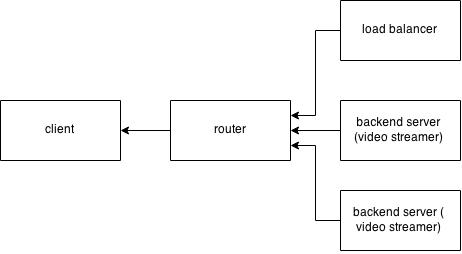
\includegraphics[width=0.4\textwidth]{raspberry pi setup.jpg}
\caption{Setup}
\label{fig:setup} %always place your label after your caption!
\end{figure}

\begin{table}[H]
	\centering \caption{Variables}
	\begin{tabular}{|c|} \hline
		\textbf{Input}  \\ \hline
		Data from SD card \\ \hline
		Data from Internet \\ \hline
		Electrical Power \\ \hline
		Cooling \\ \hline
		Measurement tools \\ \hline
		\textbf{System}  \\ \hline
		Operating system (Raspbian) \\ \hline
		Measurement software \\ \hline
		Processing power \\ \hline
	\textbf{Output} \\ \hline
		data  over network (video stream)\\ \hline
		data over HDMI \\ \hline
	\end{tabular}
	\label{tab:variables}

\end{table}
The system will make use of several variables~\ref{tab:variables}. We can distinguish three types which we need to keep in our mind during the research. We have input variables that define the input. The system has not a lot of variables, because you can choose for example a operating system, but not change the software in the operating system. By using the software of the system we can get the different result in the output variables. 

\section{Planning}

\begin{table}[H]
	\centering \caption{Planning}
\begin{tabular}{|c|c|c|} \hline
		\textbf{Week} & \textbf{Start Date} & \textbf{Activity} \\ \hline 
		6-13& 6 Feb& Collect literature and software\\ \hline 
		12& 16 March& Deadline peer review and proposal \\ \hline
		14& 23-30 March & \textbf{Deadline proposal} \\ \hline
		15 & 23-30 March &  \textbf{Accept Reject proposal} \\ \hline
		15-14& 30 March& Start building test environment \\ \hline
		16& 6 April & Answer subquestion 1  \\ \hline
		17& 13 April & Answer subquestion 2\\ \hline
		18& 21 April & Answer subquestion 3\\ \hline
		16-18 & 6 April  & working on test environment \\ \hline
		17& 1 May  & Answer subquestion 4 \\ \hline
		18& 4 May & conclusion and check coherency \\ \hline
		19& 11 May & Finalize paper \\ \hline
		22& 1 June &  \textbf{Deadline paper} \\ \hline
		23-25& 8 june & presentation preperation \\ \hline
		26 & 22 June & \textbf{Conference} \\ \hline
		\end{tabular}

		\label{tab:planning}
\end{table}
Here above is the table~\ref{tab:planning}. The main research question is split up into several sub questions. These subquestions have each one week for answering. After that there is time to write the conclusion and answer the main question. Then there is still some time left to finalize the paper. 

\section{State of the Art}
The amount of cloud computing services is increasing fast \cite{armbrust:2009}. Despite the attention
from the research community, research and development of
Cloud Computing services is still in it's early days~\cite{tso:2013}. Today there is a lot of customers that use video streaming and this will become even more. Customers want to have everything has to be accessible through the network around the clock \cite{youseff:2008}. One thing that people want on demand are there film series. Currently Netflix has 30\% of the downstream in the United States~\cite{computer-networking}. This downstream is huge and that means that there is optimization in this branch possible. To make the video on demand service of Netflix possible they use servers from Amazon. 

The Raspberry Pi is made for research and education purposes \cite{raspberry-pi}. The Raspberry Pi is a cheap device costing around 40 euro. It has a power consumption of only three watt and has quite good processor. For this reason it might be very useful for small scale cloud computing. The raspberry Pi is a small device and is excellent for a lot of small devices in a relatively small place. The Raspberry Pi doesn't use cooling and it can be used for very rapid elasticity and on-demand self-service. Because of it's cooling features and low power consumption it might be a good alternative for the nowadays high power consuming data centers. The raspberry pi is really small so it is a lot easier to place extra pi in a data center compared to a normal server. The Raspberry Pi has one drawback and that is that the processing power is relatively low. By using load balancing there will be taken a look at what load balancing techniques are successful for the Raspberry pi. 

In this research we will make a small raspberry cloud to do research on video streaming using HTTP. This will be done using the design Science method proposed by Hevner~\cite{hevner:2007}.  This research will try to find out if the raspberry has enough processing power and bandwidth to be a suitable streamer to multiple web clients. The cloud performance can now be better researched, because everything is at one location and the information about what processes are running on the pi are well defined. In this way we can take a better look at algorithms used in video streaming. This is mostly because there is not a lot of overhead. 

\bibliographystyle{abbrv}
\bibliography{sigproc}  % sigproc.bib is the name of the Bibliography in this case
% You must have a proper ".bib" file
%  and remember to run:
% latex bibtex latex latex
% to resolve all references
%
% ACM needs 'a single self-contained file'!
%
\vspace{50 mm}
\newpage
%APPENDICES are optional

\end{document}
